% This is part of Un soupçon de mathématique sans être agressif pour autant
% Copyright (c) 2014-2015
%   Laurent Claessens
% See the file fdl-1.3.txt for copying conditions.


% This is part of Un soupçon de mathématique sans être agressif pour autant
% Copyright (c) 2015
%   Laurent Claessens
% See the file fdl-1.3.txt for copying conditions.

%--------------------------------------------------------------------------------------------------------------------------- 
\subsection*{Activité : voyages en bus}
%---------------------------------------------------------------------------------------------------------------------------

Un chauffeur de bus effectue la navette entre le camping et la plage. Il est chargé de prendre note du nombre de passagers transporté chaque jour, afin que la compagnie de bus puisse savoir le nombre de bus sur la ligne est adéquat. Voici ses résultats :
\begin{equation}
\begin{array}[]{ccccccccccc}
52& 46& 32& 47& 20& 31& 26& 32& 40& 31& 57\\
33& 41& 17& 44& 39& 7& 36& 43& 51& 24& 23\\
44& 51& 34& 44& 54& 35& 49& 30& 56&
\end{array}
\end{equation}

\begin{enumerate}
    \item
 Combien de voyages a-t-il effectués au total ?
 \item
 Quel est le nombre minimum de passagers transportés pour un voyage ? Le maximum ?
\item
 Combien de voyages a-t-il effectués avec un nombre de passagers compris entre 41 (inclus) et 50 ?
\item
 Pour présenter le résultat de son travail à son patron, il aimerait réaliser un tableau et un histogramme permettant de visualiser facilement la répartition globale. Comment faire ?
\end{enumerate}

De \cite{NRHooXFvgpp5}

\vfill


Les feuilles suivantes sont à distribuer aux élèves. Elles proviennent de \cite{NRHooXFvgpp5} (licence GNU-FLD 1.1, surement compatible avec la 1.3 que j'utilise).


\begin{center}
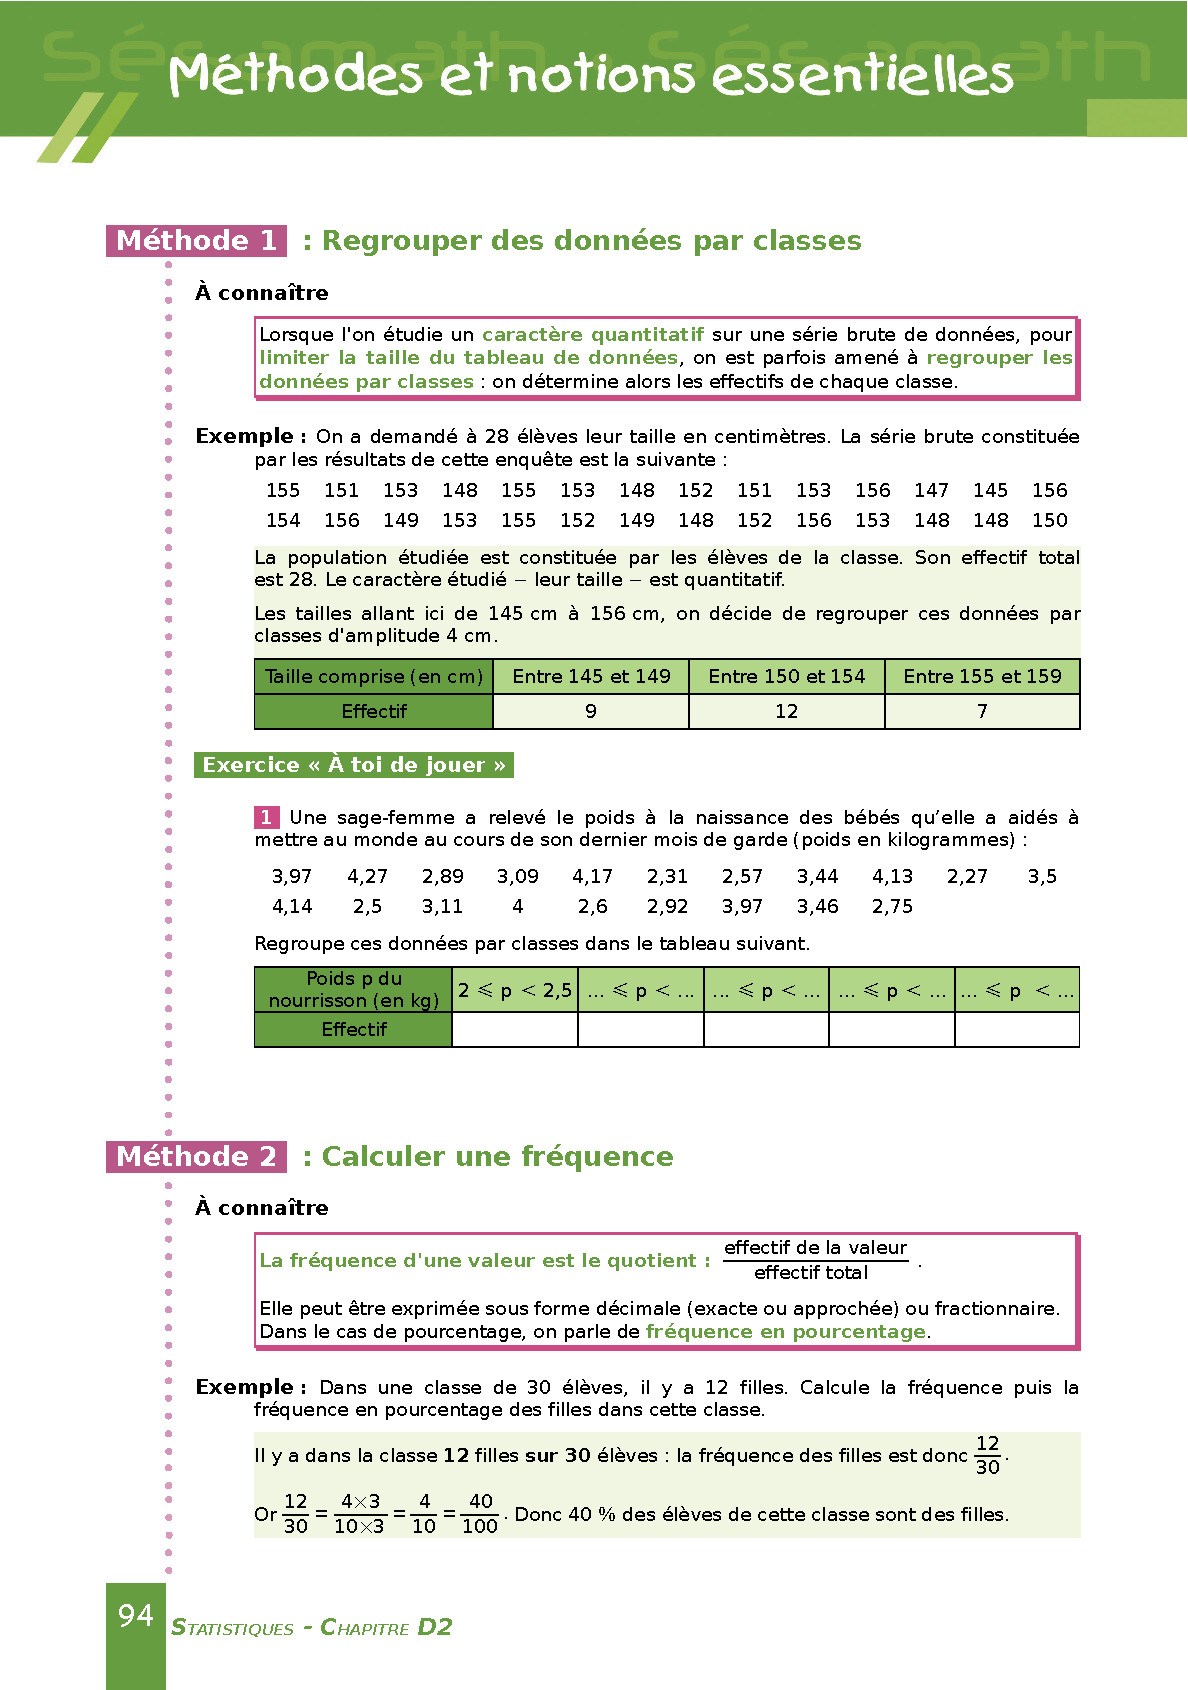
\includegraphics{sesamath5p94.pdf}
\end{center}
\begin{center}
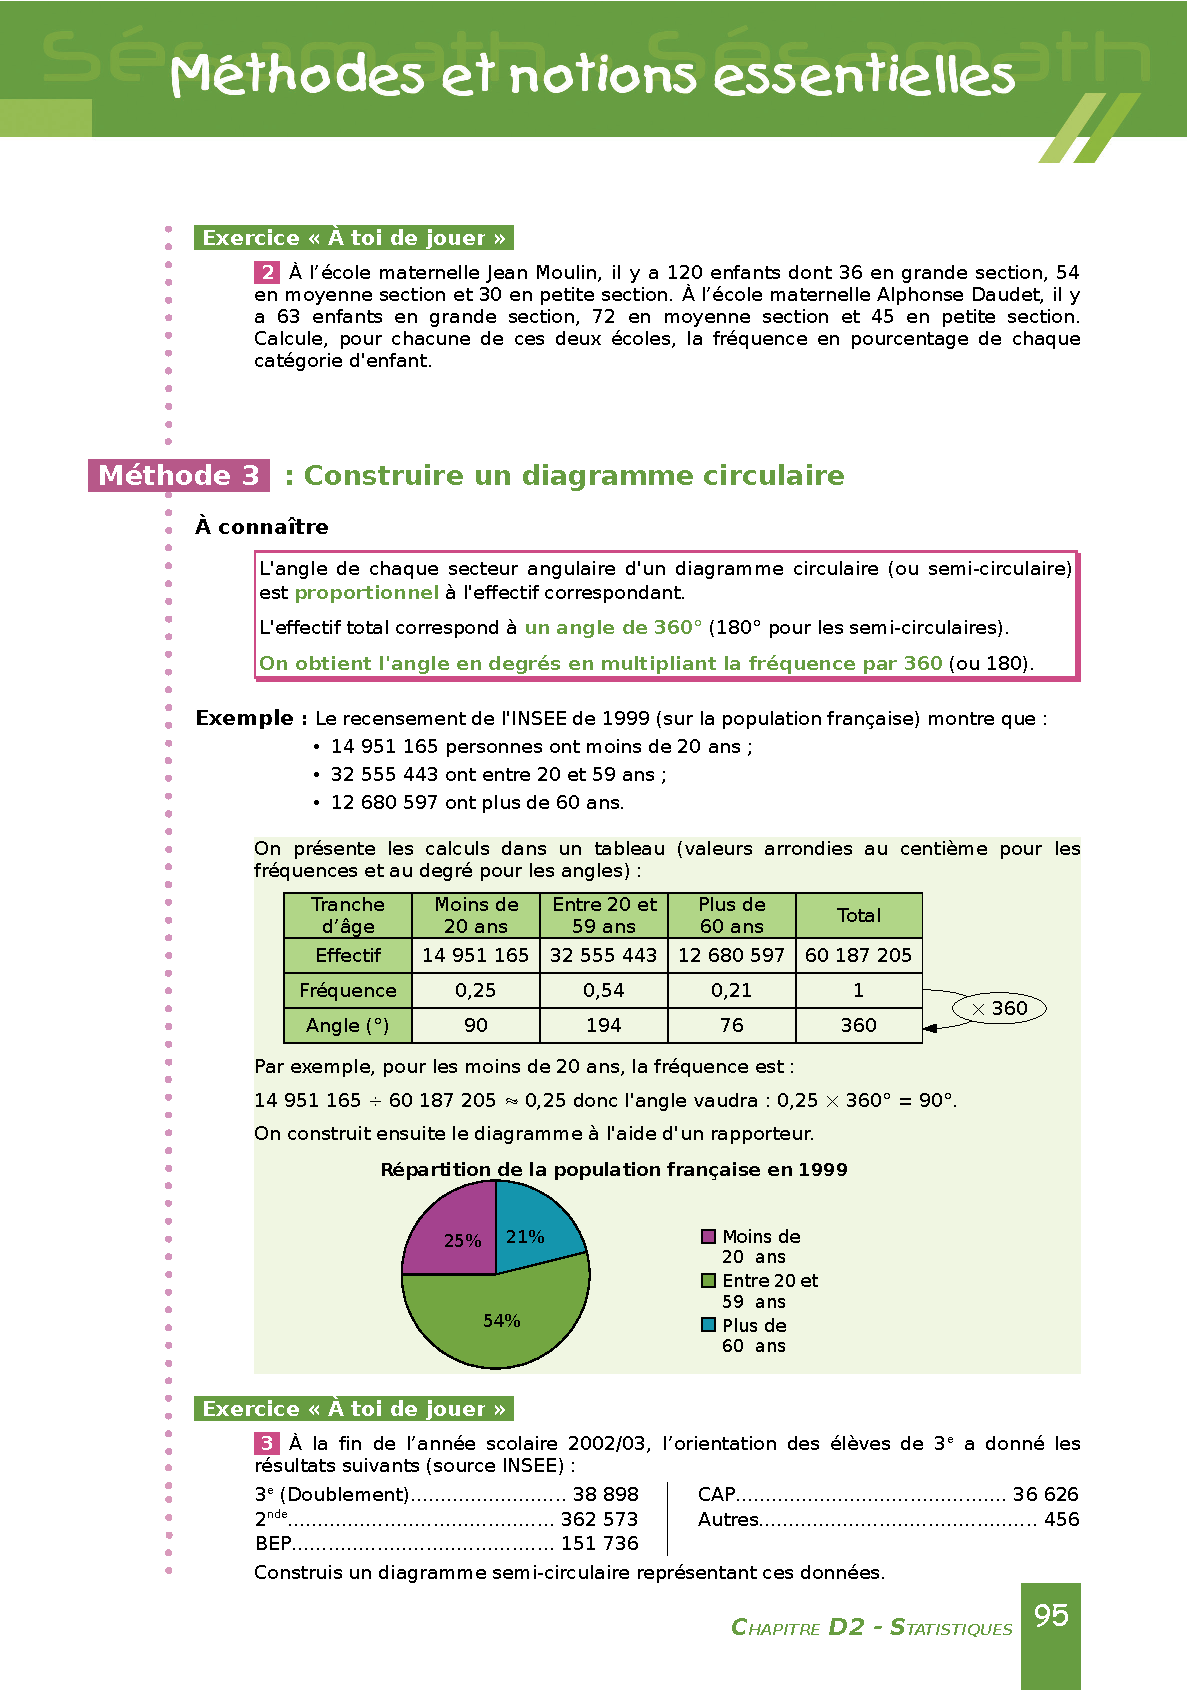
\includegraphics{sesamath5p95.pdf}
\end{center}


%+++++++++++++++++++++++++++++++++++++++++++++++++++++++++++++++++++++++++++++++++++++++++++++++++++++++++++++++++++++++++++ 
\section{Exemples : les devoirs}
%+++++++++++++++++++++++++++++++++++++++++++++++++++++++++++++++++++++++++++++++++++++++++++++++++++++++++++++++++++++++++++

Quelque statistiques sur les devoirs.

\vfill

Pour les 5A :

% les graphes viennent de phystricksTYIooYKqeNv.py

\begin{center}
   \input{Fig_CXWooOMPOQT.pstricks}
\end{center}

\vfill

Pour les 5B

\begin{center}
   \input{Fig_PJQooTWPTXV.pstricks}
\end{center}


Le couplage barème/compétences du DS numéro 6, 5A :

\begin{center}
   \input{Fig_TLEXooPDNwLRooONE.pstricks}
\end{center}

Le couplage barème/compétences du DS numéro 6, 5B :

\begin{center}
   \input{Fig_TLEXooPDNwLRooTWO.pstricks}
\end{center}
